\subsection{Sprint 4: Using real money}
With the implementation so far tested and polished, the time had come to implement our final feature. 
The last major challenge remaining at this point was linking the virtual marketplace to the real world.
So far users can trade their digital commodities for an amount of virtual currency.
The problem was that this currency had no actual value, since the only way of obtaining it was by trading it for reputation points.
So the marketplace at this point would consist out of people selling reputation points and others that do not have the means to acquire their own points, trying to buy them.
Sadly there would be no transactions made since no one had any virtual currency to make the first trade.
The solution to this problem is to allow users to use real money to either buy the virtual currency or use that money directly in the transaction.

\subsubsection{Usage of virtual currency}
Virtual currency is a great way to keep the identities of users hidden when making financial transactions. 
The problem this structure brings is that it requires a way to verify whether the digital money is actually real. 
When not using a central entity that governs the transactions, it becomes very difficult to tell where money came from and whether the balances of users are not tempered with.
There are of course solutions to this.

For example, you could implement a block-chain structure like BitCoin has made \cite{bitcoin}.
With this the whole user-base has to agree on a certain chain of transactions.
To achieve this, it is required to have every user communicate with every other user what transactions are made.
This way of regular broadcasting scales terribly and is the reason Tsukiji switched to a gossip model.

The solution for Tsukiji was to leave the idea of virtual currency completely. 
If users can use existing payment options, we no longer have to worry about security en legitimacy issues that payments bring.
The only thing that is required of Tsukiji is to link one peer to another peer and allow an easy way to perform the transaction.
The privacy issue is now brought back to the user. 
If they want to make anonymous transactions, they will have to create a separate account to make and receive transactions, that is not linked to their identity. 

\subsubsection{Online banking}
To use real money we required third party software to handle payments for us. 
After some research two options had our preference: iDeal and Paypal.
Sadly the iDeal API had a constraint that it only allowed users to give money to a business and not from person to person.
This would mean that every user has to create a business-account and have it approved by iDeal, just to make payments in Tsukiji.
As this is not deemed feasible, we chose to use Paypal instead.
\begin{figure}[H]
  \centering
  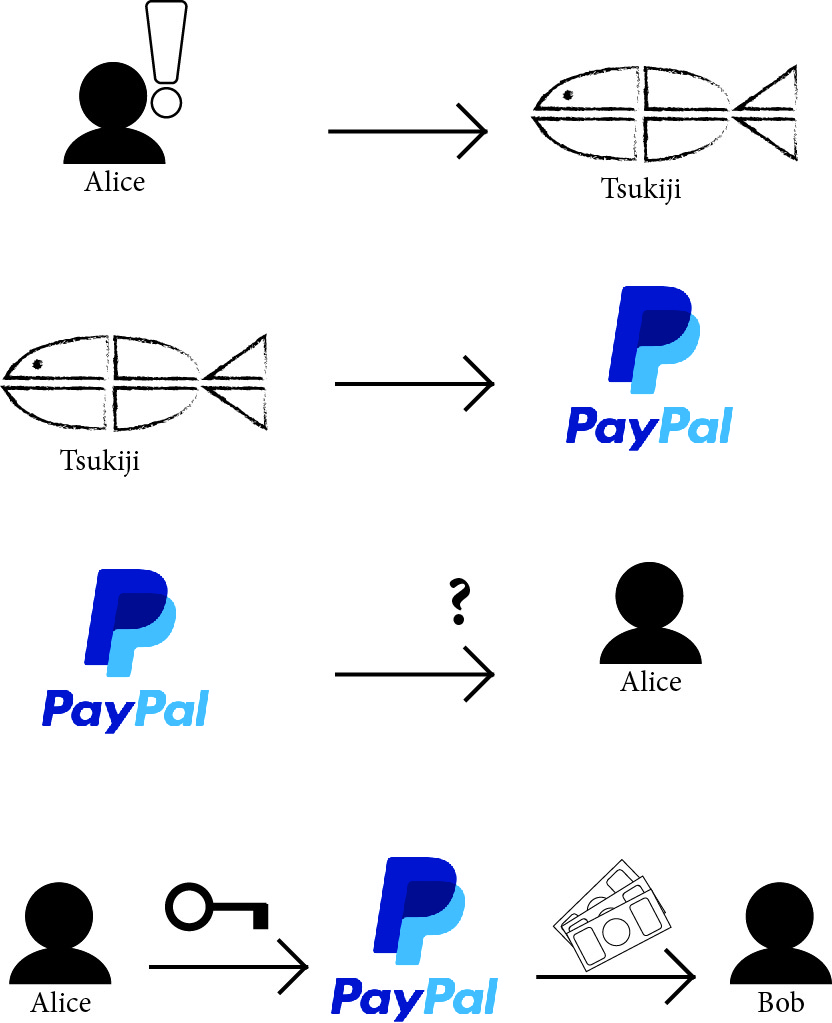
\includegraphics[width=\linewidth]{paypal-payment}
  \caption{Alice finds an interesting item on Tsukiji. Tsukiji then aks the PayPal API to create an authorisation page. This page asks Alice for het login details and then verifies the transaction, sending the money from Alice's paypal account to Bob's.}
  \label{paypal_pay}
\end{figure}
\newpage
The Paypal API\cite{paypal} offers many ways to create, send and verify transactions.
While poorly documented, there is a python integration that uses http calls with JSON objects to communicate with the Paypal servers.
The current implementation in Tsukiji creates a payment that has the amount (in euros) and the recipient pre-filled whenever a trade is made.
All the user has to do now, is fill in their login details on the Paypal page that opens automatically to authorise the transaction.
The full process is depicted in Figure \ref{paypal_pay}.
This way the user does not need to trust Tsukiji with their Paypal credentials and does not even need to know the address of the person they are about to pay.
This approach keeps Tsukiji decentralised as well, since the Paypal service is not part of the implementation of Tsukiji itself.

Tsukiji now has a way for users to pay eachother that is reliable but leaves itself unaccountable for any errors in transactions.
Users only have to trust Paypal for their transactions, which complies with the zero-trust ideology of a decentralised system.
